
%	Event reconstruction

\section{Event reconstruction}\label{Section_Reconstruction}
\Headerfooter{Event reconstruction}
\subsection{Vertex reconstruction}\label{Subsec_vertex_rec}
\vs\hs
A charged particle with the energy of $\mathcal{O}$(10)~MeV travel a few centimeters in water.
Since vertex resolution is worse than track length of the charged particle due to the detector size and time resolution of PMTs, track length of the charged particle can be treated as a point.
Vertex is reconstructed by using a maximum-likelihood method.
The likelihood function is defined as
\begin{eqnarray}
	\mathcal{L}(\bm{x},t_{0}) &=& \sum_{i=1}^{N_{\rm hit}} \log P(t_{{\rm res},i}), \\
	t_{{\rm res},i}           &=& t_{i} - t_{0} - {|\bm{x} - \bm{h}_{i}| \over c},
\end{eqnarray}
where $\bm{x} = (x,y,z)$ is the candidate vertex, $t_{0}$ is the time when a charged particle was generated, $N_{\rm hit}$ is the number of hit PMTs, $t_{{\rm res},i}$ is the timing residual, $P(t_{{\rm res},i})$ is the probability density function for $t_{{\rm res},i}$, $t_{i}$ is the PMT's hit time, $\bm{h}_{i}$ is the position of hit PMT, and $c$ is the group velocity of light in water.
$t_{0}$ is fitted to minimize all $t_{{\rm res},i}$.
Figure~\ref{Recons_SK_coordinate} and Figure~\ref{Recons_PDF_vertex} shows the definition of the SK detector coordinate system~\cite{2016Abe} and the probability density function for $t_{{\rm res},i}$~\cite{2023HaradaPhD}, respectively.
Moreover, vertex resolution for SK-I, II, III, and IV is shown in Figure~\ref{Recons_Res_vertex}~\cite{2016Abe}.

\begin{figure}[h]
	\centering
	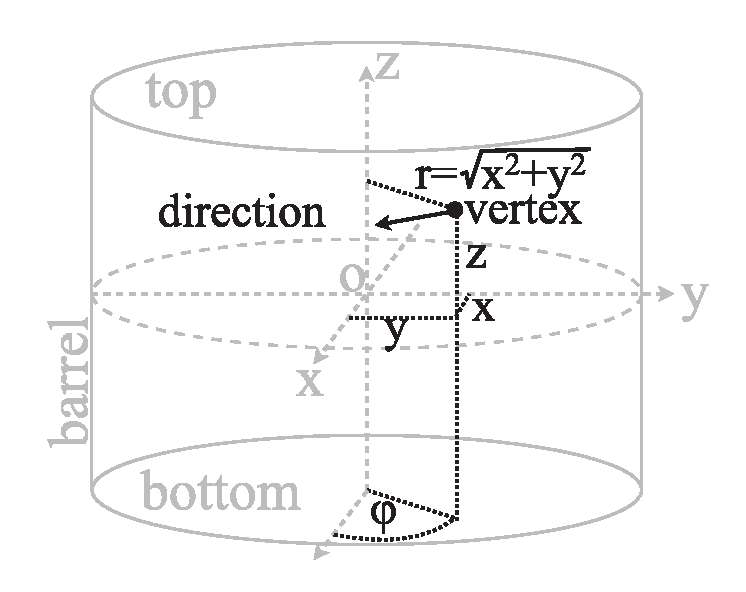
\includegraphics[width=6cm]{Figures/Reconstruction/SK_coordinate}
	\caption[Definition of the SK detector coordinate system]{
	Definition of the SK detector coordinate system~\cite{2016Abe}.
	}\label{Recons_SK_coordinate}
\end{figure}

\begin{figure}[h]
	\centering
	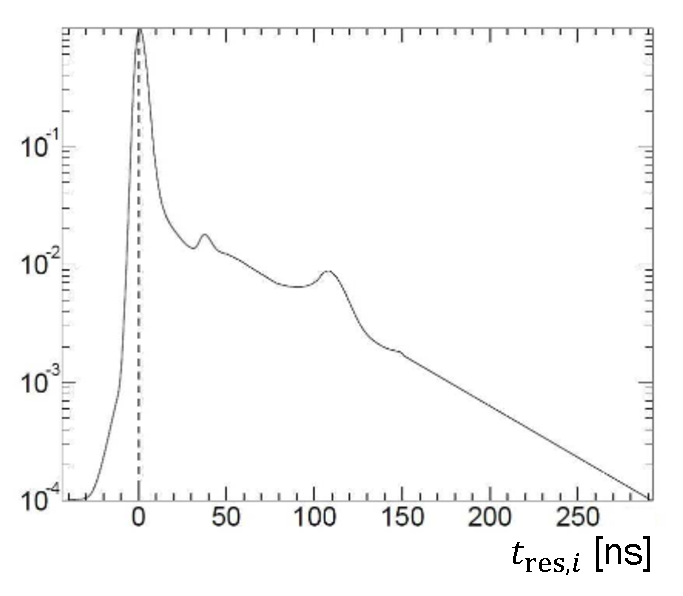
\includegraphics[width=8cm]{Figures/Reconstruction/PDF_vertex}
	\caption[Probability density function for $t_{{\rm res},i}$]{
	Probability density function for $t_{{\rm res},i}$~\cite{2023HaradaPhD}.
	Peaks around 40~ns and 110~ns come from after pulses of PMTs.
	}\label{Recons_PDF_vertex}
\end{figure}

\begin{figure}[tbp]
	\centering
	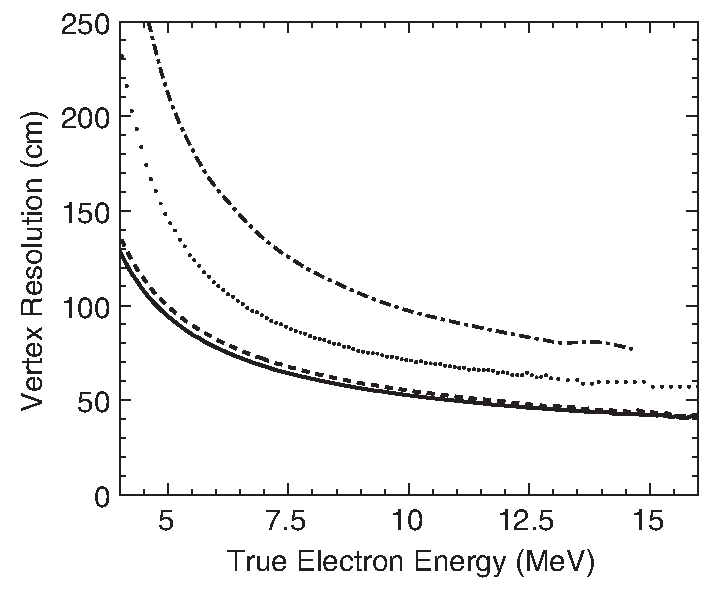
\includegraphics[width=8cm]{Figures/Reconstruction/Res_vertex}
	\caption[Vertex resolution for SK-I, II, III, and IV]{
	Vertex resolution for SK-I, II, III, and IV~\cite{2016Abe}.
	Dotted, dashed-dotted, dashed, and solid line shows that for SK-I, II, III, and IV, respectively.
	}\label{Recons_Res_vertex}
\end{figure}

\hs
The vertex reconstruction goodness, which is a parameter that indicates whether the vertex reconstruction is done well or not, is defined as
\begin{eqnarray}
	g_{\rm vtx} = {\displaystyle \sum_{i=1}^{N_{\rm hit}} \bigg[\exp\bigg\{-\bigg({t_{{\rm res},i} \over \sqrt{2}\omega}\bigg)^{2}\bigg\}\exp\bigg\{-\bigg({t_{{\rm res},i} \over \sqrt{2}\sigma}\bigg)^{2}\bigg\}\bigg] \over \displaystyle \sum_{i=1}^{N_{\rm hit}} \exp\bigg\{-\bigg({t_{{\rm res},i} \over \sqrt{2}\omega}\bigg)^{2}\bigg\}},
\end{eqnarray}
where $\omega$ is the resolution of the $t_{{\rm res},i}$ distribution and $\sigma$ is the timing resolution of PMTs.
The range of $g_{\rm vtx}$ is from 0 to 1, and the value is close to 1 when the vertex reconstruction is done well.





\subsection{Direction reconstruction}\label{Subsec_direction_rec}
\vs\hs
After determining the vertex, direction is reconstructed.
Direction is reconstructed by using a maximum-likelihood method with hit PMTs within 20~ns.
The likelihood function is defined as
\begin{eqnarray}
	\mathcal{L}(\bm{d}) = \sum_{i=1}^{N_{20}} \bigg[\log f(\cos\Theta_{i},E) \times {\cos\theta_{i} \over a(\theta_{i})}\bigg],
\end{eqnarray}
where $\bm{d}$ is the candidate direction, $N_{20}$ is the number of hit PMTs within 20~ns, $\Theta_{i}$ is the angle between the candidate direction and the direction from the reconstructed vertex to the position of hit PMT, $f(\cos\Theta_{i},E)$ is the probability density function for $\cos\Theta_{i}$ depending on the energy $E$, $\theta_{i}$ is the angle between the direction from the reconstructed vertex to the position of hit PMT and the direction in which the hit PMT is oriented, and $a(\theta_{i})$ is the correction function of PMT acceptance.
$a(\theta_{i})$ is defined as
\begin{eqnarray}\label{Recons_Eq_a_theta}
	a(\theta_{i}) = 0.205 + 0.524\cos\theta_{i} + 0.390\cos^{2}\theta_{i} - 0.132\cos^{3}\theta_{i}.
\end{eqnarray}
Figure~\ref{Recons_PDF_direction} shows the probability density function for $\cos\Theta_{i}$ depending on the energy $E$~\cite{2011Abe}.
Moreover, Figure~\ref{Recons_Res_direction} shows the angular resolution for SK-I and SK-III~\cite{2011Abe}.

\begin{figure}[tbp]
	\centering
	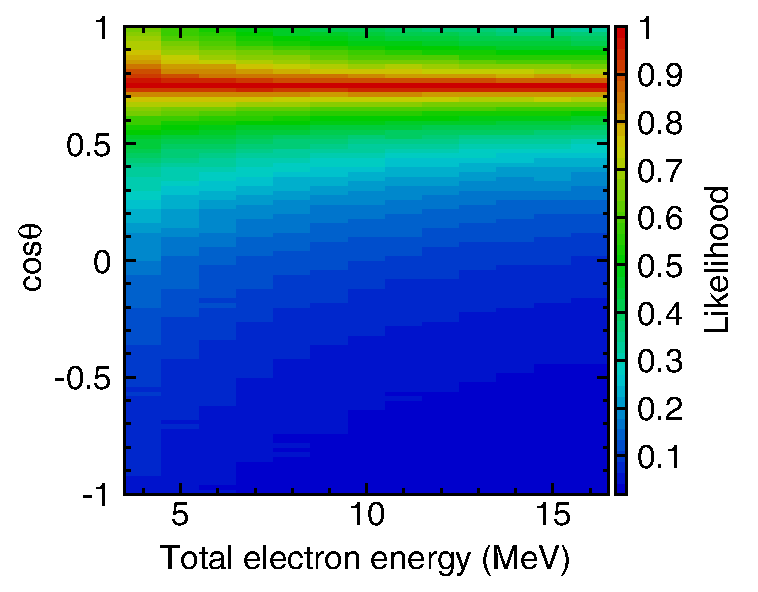
\includegraphics[width=8cm]{Figures/Reconstruction/PDF_direction}
	\caption[Probability density function for $\cos\Theta_{i}$ depending on the energy $E$]{
	Probability density function for $\cos\Theta_{i}$ depending on the energy $E$~\cite{2011Abe}.
	}\label{Recons_PDF_direction}
\end{figure}

\begin{figure}[tbp]
	\centering
	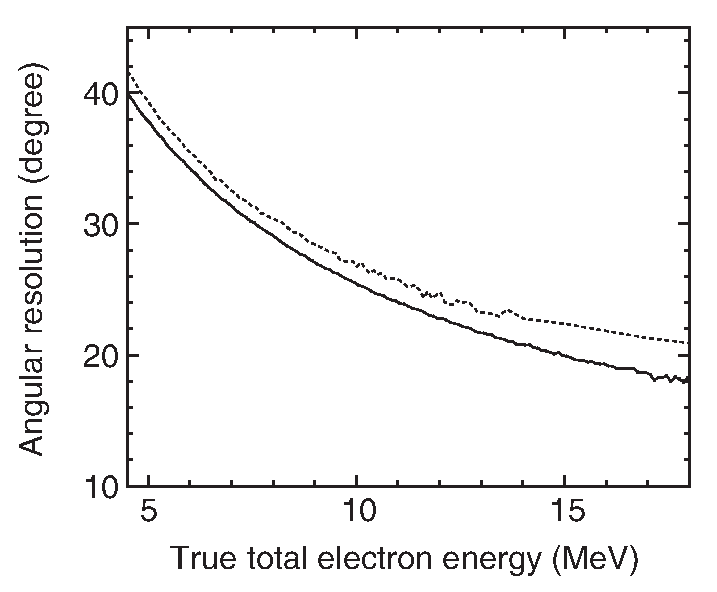
\includegraphics[width=8cm]{Figures/Reconstruction/Res_direction}
	\caption[Angular resolution for SK-I and SK-III]{
	Angular resolution for SK-I and SK-III~\cite{2011Abe}.
	Dashed and solid line shows that for SK-I and SK-III, respectively.
	}\label{Recons_Res_direction}
\end{figure}

\hs
The direction reconstruction goodness, which is a parameter that indicates whether the direction reconstruction is done well or not, is defined as
\begin{eqnarray}
	g_{\rm dir} = {1 \over 2\pi}\bigg\{{\rm max}\bigg(\phi_{i} - {2\pi \times i \over N_{\rm hit}}\bigg) - {\rm min}\bigg(\phi_{i} - {2\pi \times i \over N_{\rm hit}}\bigg)\bigg\},
\end{eqnarray}
where $\phi_{i}$ is the azimuthal angle of the $i$-th hit PMT.
The range of $g_{\rm dir}$ is from 0 to 1, and the value is close to 0 when the direction reconstruction is done well.





\subsection{Energy reconstruction}
\vs\hs
Energy is reconstructed by using $N_{\rm eff}$, which does not depend on vertex, direction, the number of bad-channel PMTs, water transparency, and relative quantum efficiency (QE) of each PMT.
$N_{\rm eff}$ is defined as
\begin{eqnarray}\label{Eq_Recons_Neff}
	N_{\rm eff} = \sum_{i=1}^{N_{50}} \biggl[(X_{i} + \epsilon_{\rm tail} - \epsilon_{\rm dark}) \times {N_{\rm all} \over N_{\rm alive}} \times {S(0,0) \over S(\theta_{i},\phi_{i})} \times \exp\biggl({r_{i} \over L_{\rm eff}^{i}}\biggr) \times {1 \over QE_{i}}\biggr],
\end{eqnarray}
where $N_{50}$ is the number of hit PMTs within 50~ns.
Parameters shown in Equation~(\ref{Eq_Recons_Neff}) is described below.\\

\textbf{$X_{i}$ : Correction for multiple hits}\\
\hs
When an event occur at the edge of fiducial volume or an event is caused by a charged particle with high energy, multiple photons may hit a PMT nearby the vertex.
The multiple hits are corrected by using $X_{i}$ defined as
\begin{eqnarray}
	X_{i} &=&
	\left\{
	\begin{array}{ll}
		\displaystyle {\log\{1/(1 - n_{i}/N_{i})\} \over n_{i}/N_{i}} & (n_{i}/N_{i} < 1) \\
		3.0                                                           & (n_{i}/N_{i} = 1)
	\end{array} \right.,
\end{eqnarray}
where $N_{i}$ is the number of PMTs adjacent to the hit PMT and $n_{i}$ is the number of hits in the adjacent PMTs.\\

\textbf{$\epsilon_{\rm tail}$ : Correction for scattering and reflection}\\
\hs
Cherenkov photons scattering in water or reflecting at the surface of PMT or black sheet may hit a PMT at time out of a time width of 50~ns.
The effects of scattering and reflection are corrected by using $\epsilon_{\rm tail}$ defined as
\begin{eqnarray}
	\epsilon_{\rm tail} = {N_{100} - N_{50} - N_{\rm alive} \times R_{\rm dark} \times 50\,{\rm ns} \over N_{50}},
\end{eqnarray}
where $N_{100}$ is the number of hit PMTs within 100~ns, $N_{\rm alive}$ is the number of alive PMTs and $R_{\rm dark}\,({\rm hits}/{\rm ns})$ is the dark-noise rate at a period.\\

\textbf{$\epsilon_{\rm dark}$ : Correction for dark-noise hits}\\
\hs
Hits caused by PMT dark noise may enter the time width of 50~ns.
The dark-noise hits, which are not originated from Cherenkov photons, are corrected by using $\epsilon_{\rm dark}$ defined as
\begin{eqnarray}
	\epsilon_{\rm dark} = {N_{\rm alive}\times R_{\rm dark} \times 50\,{\rm ns} \over N_{50}} \times {R_{\rm dark}^{i} \over \displaystyle \sum_{i=1}^{N_{50}} {R_{\rm dark}^{i} \over N_{50}}},
\end{eqnarray}
where $R_{\rm dark}^{i}\,({\rm hits}/{\rm ns})$ is the dark-noise rate of the $i$-th hit PMT at a period.\\

\textbf{$N_{\rm all}/N_{\rm alive}$ : Correction for bad-channel PMTs}\\
\hs
If there is a PMT that does not work properly, the number of hits would be underestimated and energy would not be reconstructed correctly.
The effects of bad-channel PMTs are corrected by multiplying $N_{\rm all}/N_{\rm alive}$, where $N_{\rm all}\,(= 11{,}129)$ is the number of all PMTs.\\

\textbf{$S(0,0)/S(\theta_{i},\phi_{i})$ : Correction for change of photo coverage by the incident angle of photon}\\
\hs
Photo coverage changes depending on the incident angle of a Cherenkov photon.
This effect is corrected by using the correction function $S(\theta_{i},\phi_{i})$.
Figure~\ref{Recons_PMT_theta_phi} and Figure~\ref{Recons_PMTCorrFunc} show the definition of the incident angle and distributions of correction function $S(\theta_{i},\phi_{i})$ for barrel PMTs and top and bottom PMTs, respectively.\\

\begin{figure}[h]
	\centering
	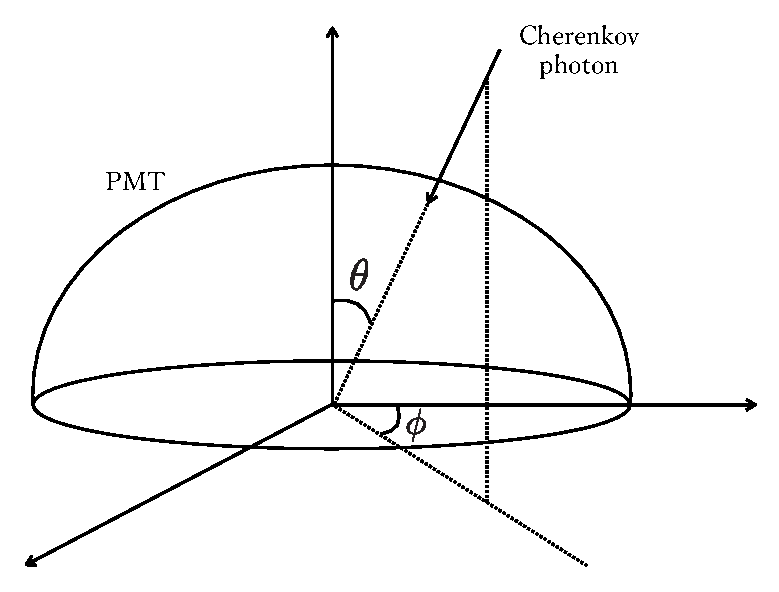
\includegraphics[width=8cm]{Figures/Reconstruction/PMT_theta_phi}
	\caption[Definition of the incident angle]{
	Definition of the incident angle~\cite{2021ShinokiMas}.
	}\label{Recons_PMT_theta_phi}
\end{figure}

\begin{figure}[h]
	\centering
	\includegraphics[width=16cm]{Figures/Reconstruction/PMTCorrFunc}
	\caption[Distributions of correction function $S(\theta_{i},\phi_{i})$ for barrel PMTs and top and bottom PMTs]{
	Distributions of correction function $S(\theta_{i},\phi_{i})$ for barrel PMTs (left) and top and bottom PMTs (right)~\cite{2021ShinokiMas}.
	}\label{Recons_PMTCorrFunc}
\end{figure}

\textbf{$\exp(r_{i}/L_{\rm eff}^{i})$ : Correction for water transparency}\\
\hs
Cherenkov photons may be scattered or absorbed in water before arriving at a PMT.
The probability that a Cherenkov photon arrives at a PMT can be written as $\exp(-r_{i}/L_{\rm eff}^{i})$, where $r_{i}$ is the distance from the vertex to a hit PMT and $L_{\rm eff}^{i}$ is the effective attenuation length, which is described below.
Therefore, the effect of water transparency is corrected by multiplying $\exp(r_{i}/L_{\rm eff}^{i})$.\\
\hs
$L_{\rm eff}^{i}$ is expressed as
\begin{eqnarray}
	L_{\rm eff}^{i} = -{r_{i} \over {\rm ln}\Bigg[\displaystyle \int_{\lambda_{\rm min}}^{\lambda_{\rm max}} w_{0}(\lambda)\exp\{-\sigma_{i}(\lambda) \times r_{i}\} d\lambda\Bigg]},
\end{eqnarray}
where $\lambda_{\rm min} = 300\,{\rm nm}$, $\lambda_{\rm max} = 650\,{\rm nm}$, $w_{0}(\lambda)$ is the probability density function for wavelength $\lambda$ of Cherenkov photons (shown in Figure~\ref{Recons_PDF_wavelength}), and $\sigma_{i}(\lambda)$ is the cross section with water when a Cherenkov photon travels a distance $r_{i}$.
$\sigma_{i}(\lambda)$ is expressed as
\begin{eqnarray}
	\sigma_{i}(\lambda) = \alpha_{\rm abs}(\lambda)\bigg\{1 + \beta\bigg(z + {1 \over 2}r_{i} \times dz_{i}\bigg)\bigg\} + C_{\rm sca}\{\alpha_{\rm sym}(\lambda) + \alpha_{\rm asy}(\lambda)\},
\end{eqnarray}
where $z$ is the z position of the vertex, $dz_{i}$ is the z component of direction to the hit PMT, and $C_{\rm sca} (\sim 0.44)$ is the correction factor of the scattering effect.
$C_{\rm sca}$ was estimated to minimize the position dependence of $N_{\rm eff}$ using the SK detector simulation.
$\alpha_{\rm abs}(\lambda)$, $\alpha_{\rm sym}(\lambda)$, and $\alpha_{\rm asy}(\lambda)$ are the attenuation coefficients of absorption, symmetric scattering, and asymmetric scattering at wavelength $\lambda$, respectively, and $\beta$ is the parameter indicating the degree of z dependence in water quality.
Details about $\alpha_{\rm abs}(\lambda)$, $\alpha_{\rm sym}(\lambda)$, $\alpha_{\rm asy}(\lambda)$, and $\beta$ are described in Section~\ref{Subsubsec_Water}.

\begin{figure}[h]
	\centering
	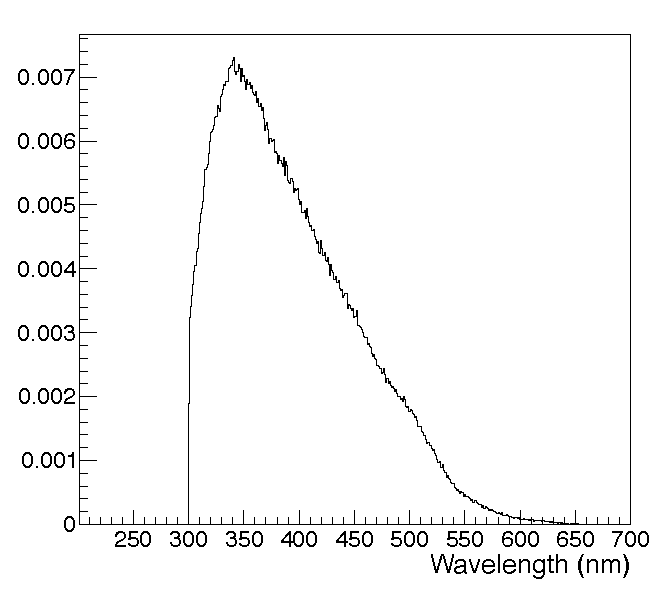
\includegraphics[width=8cm]{Figures/Reconstruction/PDF_wavelength}
	\caption[Probability density function for wavelength $\lambda$ of Cherenkov photons]{
	Probability density function for wavelength $\lambda$ of Cherenkov photons~\cite{2021ShinokiMas}.
	}\label{Recons_PDF_wavelength}
\end{figure}

\textbf{$1/QE_{i}$ : Correction for relative QE of each PMT}\\
\hs
QE differs for each PMT.
The effect of QE is corrected by multiplying $1/QE_{i}$, where $QE_{i}$ is the relative QE of the hit PMT.
Details about $QE_{i}$ are described in Section~\ref{Subsubsec_QE}.\\
\\
\hs
Visible energy of the prompt signal ($E_{\rm vis}$) is determined by using $N_{\rm eff}$.
Relation between $E_{{\rm vis}}$ and $N_{\rm eff}$ is expressed as 
\begin{eqnarray}
	E_{\rm vis} =
	\left\{
	\begin{array}{ll}
		\displaystyle \sum_{i=0}^{5} p_{i}(N_{\rm eff})^{i}                                                                                 & (N_{\rm eff} \leq N_{\rm thr}) \\
		\displaystyle \sum_{i=0}^{5} p_{i}(N_{\rm thr})^{i} + (N_{\rm eff} - N_{\rm thr}) \times \sum_{i=1}^{5} ip_{i}(N_{\rm thr})^{i - 1} & (N_{\rm eff} > N_{\rm thr})
	\end{array} \right..
\end{eqnarray}
The values of $p_{i}$ and $N_{\rm thr}$ are summarized in Table~\ref{tab:Recons_Neff}.

\begin{table}[H]
	\centering
	\caption[Values of $p_{i}$ and $N_{\rm thr}$]{
	Values of $p_{i}$ and $N_{\rm thr}$~\cite{2023HaradaPhD}.
	}\label{tab:Recons_Neff}
	\vs
	\begin{tabular}{cc} \hline \hline
		$p_{0}$       & $0.702$                 \\
		$p_{1}$       & $0.131$                 \\
		$p_{2}$       & $-2.35 \times 10^{-4}$  \\
		$p_{3}$       & $2.640 \times 10^{-6}$  \\
		$p_{4}$       & $-1.188 \times 10^{-8}$ \\
		$p_{5}$       & $1.930 \times 10^{-11}$ \\
		$N_{\rm thr}$ & $2.202 \times 10^{2}$   \\ \hline \hline
	\end{tabular}
\end{table}





\newpage

